\input{/Users/lsb/TMACROS/slideshead.tex}


\usepackage{xfrac}
\usepackage{etex}
\usepackage{tikz}
\usetikzlibrary{snakes}
\usetikzlibrary{patterns}
\usepackage{wrapfig}
\usepackage{stackrel}
\usepackage{array}
\usepackage[all,cmtip]{xy}
\xyoption{2cell}
\usepackage{multicol}
\usepackage{pgfplots}
\usepgfplotslibrary{patchplots}

\usepackage{euler}




\input{/Users/lsb/TMACROS/myabv.mac}
\input{/Users/lsb/TMACROS/LSBmacros.mac}


%------ using color ---------------------------------------------------------
\usepackage{xcolor}
\definecolor{indigo}{rgb}{0.29, 0.0, 0.51}
\definecolor{ggray}{rgb}{0.75, 0.75, 0.75}
\definecolor{gray}{rgb}{0.5, 0.5, 0.5}
\definecolor{dimgray}{rgb}{0.41, 0.41, 0.41}
\definecolor{antiquefuchsia}{rgb}{0.57, 0.36, 0.51}
\definecolor{goldenrod}{rgb}{.80392 .60784 .11373}
\definecolor{darkgoldenrod}{rgb}{.5451 .39608 .03137}
\definecolor{brown}{rgb}{.15 .15 .15}
\definecolor{darkolivegreen}{RGB}{.33333 .41961 .18431}
\definecolor{darkpp}{rgb}{.80392 .60784 .11373}
\definecolor{crimsonglory}{rgb}{0.75, 0.0, 0.2}

\def\gre#1{{\color{darkolivegreen}{\bf #1}}}
\def\purple#1{{\color{darkpp}{#1}}}
\def\gold#1{{\color{goldenrod}{#1}}}

\def\roxo#1{{\color{indigo}{#1}}}
\def\cinza#1{{\color{gray}{#1}}}
\def\dcinza#1{{\color{dimgray}{#1}}}

\def\crim#1{{\color{crimsonglory}{#1}}}
\def\golden#1{{\color{darkgoldenrod}{#1}}}
\def\dgold#1{{\color{darkgoldenrod}{#1}}}

\def\black{\color{black}}
\def\blue{\color{blue}}
\def\red{\color{red}}


\def\dkb#1{{\blue #1}}
\def\rdb#1{{\red #1}}

\DeclareMathOperator{\out}{\mathsf{out}}
\DeclareMathOperator{\nxt}{\mathsf{nxt}}

\def\ana#1#2{\mathopen{[\!(}#1\mathclose{)\!]}_{#2}}
\def\sana#1{\mathopen{[\!(}#1\mathclose{)\!]}}

\def\lana{ 
  [ \hspace{-0.2em} ( 
}
\def\rana{ 
   ) \hspace{-0.2em} ] 
}

\def\mop{\divideontimes}


%%%%%%%%%%%%%%%%%%%%%%%%%% REF
\def\bimmais#1{\ensuremath{\bim_+}{#1}}         % B+(X)
\def\Powmais#1{\ensuremath{\mathcal{P}_+}{#1}}         % P(X)
\def\ttot#1{#1\! \uparrow}
\def\rcb#1#2#3#4{\const{#1 \ #2 \ : \ #3 : \ #4}}
\def\tuplo#1{\mathopen{\langle}#1\mathclose{\rangle}} % <a,b,...z>
%\def\paragraph#1{\par\emph{#1}.}
\def\Vpp{\textsc{Vdm$^{\mbox{\scriptsize ++}}$}}
\def\Zpp{\textsc{Z$^{\mbox{\scriptsize ++}}$}}
\def\htmladdnormallink#1{\relax}
\def\traco{\noindent\mbox{}\hrulefill\mbox{} \\*}
\def\inT#1{{\in_{{\fun T}_{#1}}}}
\def\leqT#1{{\leq_{{\fun T}_{#1}}}}
\def\inTT#1#2#3{{\in_{{\fun T}_{#1} #2 {\fun T}_{#3}}}}
\def\leqTT#1#2#3{\leq_{{\fun T}_{#1} #2 {\fun T}_{#3}}}
\def\inTK{\in_{\fun T^{K}}}
\def\leqTK{\leq_{\fun T^{K}}}
%\newenvironment{lcbr}{\left\{\begin{array}{l}}{\end{array}\right.}
\def\rcb#1#2#3#4{#1}
\def\plift#1#2{(#2)^{#1}}
\def\punlift#1#2{(#2)_{#1}}
\def\lift#1{\stackrel.{#1}}
\def\condigual{\mathbin{\stackrel{?}{=}}}
\def\menor{\lift{\leq}}
% relations

\def\tot{\mathsf{T}}
\def\wlp#1#2{#1 \mathbin{\setminus\hskip-1.1ex\bullet} #2}

\def\rdiv{\mathbin{\setminus}}
\def\ldiv{\mathbin{/}}

\def\implied{\mathbin\Leftarrow}
\def\implies{\mathbin{\Rightarrow}}
\def\biimplies{\mathbin{\Leftrightarrow}}
\def\tfunc#1{\longrightarrow {#1}}       % total   funct.
\def\frarrow{\mathbin{\rightarrow}}

\def\compl#1{\neg{#1}}     
\def\trace#1{Tr(#1)}
\def\tracek#1{Tr^{Kl}(#1)}

\def\arrayin#1{\begin{array}{rcl}#1\end{array}}


\def\deff{\eqdef}
\def\ie{{\em i.e.\/}}
\newcommand{\specialcell}[2][c]{%
\begin{tabular}[#1]{@{}l@{}}#2\end{tabular}}


%\newcommand{\mH}{\mathcal{H}}

% de IC
\def\Act{N}
\def\rtran#1{\stackrel{#1}{\longrightarrow}}
\def\tran#1{\stackrel{#1}{\longrightarrow}}
\def\primertran#1{\stackrel{#1}{\longrightarrow'}}
\def\rra{\longrightarrow}
\def\reach#1{\stackrel{#1}{\longrightarrow}^*}
\def\pair#1{\mathopen{\langle}#1\mathclose{\rangle}}
\def\const#1{\mathopen{\langle}#1\mathclose{\rangle}}

%------------






\def\mop{\divideontimes}


%%%%%%%%%%%%%%%%%%%%%%%%%% REF
\def\bimmais#1{\ensuremath{\bim_+}{#1}}         % B+(X)
\def\Powmais#1{\ensuremath{\mathcal{P}_+}{#1}}         % P(X)
\def\ttot#1{#1\! \uparrow}
\def\rcb#1#2#3#4{\const{#1 \ #2 \ : \ #3 : \ #4}}
\def\tuplo#1{\mathopen{\langle}#1\mathclose{\rangle}} % <a,b,...z>
%\def\paragraph#1{\par\emph{#1}.}
\def\Vpp{\textsc{Vdm$^{\mbox{\scriptsize ++}}$}}
\def\Zpp{\textsc{Z$^{\mbox{\scriptsize ++}}$}}
\def\htmladdnormallink#1{\relax}
\def\traco{\noindent\mbox{}\hrulefill\mbox{} \\*}
\def\inT#1{{\in_{{\fun T}_{#1}}}}
\def\leqT#1{{\leq_{{\fun T}_{#1}}}}
\def\inTT#1#2#3{{\in_{{\fun T}_{#1} #2 {\fun T}_{#3}}}}
\def\leqTT#1#2#3{\leq_{{\fun T}_{#1} #2 {\fun T}_{#3}}}
\def\inTK{\in_{\fun T^{K}}}
\def\leqTK{\leq_{\fun T^{K}}}
\newenvironment{lcbr}{\left\{\begin{array}{l}}{\end{array}\right.}
\def\plift#1#2{(#2)^{#1}}
\def\punlift#1#2{(#2)_{#1}}
\def\lift#1{\stackrel.{#1}}
\def\condigual{\mathbin{\stackrel{?}{=}}}
\def\menor{\lift{\leq}}

\def\qiskit{\textsf{Qiskit}}
% relations

\def\tot{\mathsf{T}}
\def\wlp#1#2{#1 \mathbin{\setminus\hskip-1.1ex\bullet} #2}

\def\rdiv{\mathbin{\setminus}}
\def\ldiv{\mathbin{/}}

\def\implied{\mathbin\Leftarrow}
\def\implies{\mathbin{\Rightarrow}}
\def\biimplies{\mathbin{\Leftrightarrow}}
\def\tfunc#1{\longrightarrow {#1}}       % total   funct.
\def\frarrow{\mathbin{\rightarrow}}

\def\compl#1{\neg{#1}}     
\def\trace#1{Tr(#1)}
\def\tracek#1{Tr^{Kl}(#1)}

\def\arrayin#1{\begin{array}{rcl}#1\end{array}}



%%%%% Madeira
\newcommand{\Mod}{\mathrm{Mod}}
\newcommand{\Nom}{\mathrm{Nom}}
\newcommand{\Prop}{\mathrm{Prop}}
\def\HHL{\mathcal{HHL}}
\def\sat#1{\models_{#1}}
%\newcommand{\ST}{\mathrm{ST}}
\newcommand{\HR}{\rightharpoonup}

\def\deff{\eqdef}
\def\ie{{\em i.e.\/}}

\newcommand{\mH}{\mathcal{H}}

% de IC
\def\Act{N}
\def\rtran#1{\stackrel{#1}{\longrightarrow}}
\def\tran#1{\stackrel{#1}{\longrightarrow}}
\def\primertran#1{\stackrel{#1}{\longrightarrow'}}
\def\rra{\longrightarrow}
\def\reach#1{\stackrel{#1}{\longrightarrow}^*}
\def\pair#1{\mathopen{\langle}#1\mathclose{\rangle}}
\def\const#1{\mathopen{\langle}#1\mathclose{\rangle}}





\title{~\\ ~\\ 
	\textbf{
	A course in Quantum Computation \\ Introduction} 
	%\\ {\small (Habilitation lecture)}
	%\vspace{0.1cm}
	}
\author{~\\ ~\\ Lu\'{\i}s Soares  Barbosa \& Renato Neves\\}
\institute{
\\ 
\includegraphics[height=1.2cm]{/Users/lsb/TLOGOS/uminho.pdf}\hspace{0.5cm}
 \includegraphics[height=1cm]{/Users/lsb/TLOGOS/haslab-logo.pdf} \hspace{0.5cm}
 
\includegraphics[height=1cm]{/Users/lsb/TLOGOS/inl}\hspace{0.3cm}
 \includegraphics[height=1cm]{/Users/lsb/TLOGOS/unu-egov} 
\vspace{0.3cm}
}
%\institute{High-Assurance-Software Lab (HASLab)\\ INESC TEC \& U.Minho, Portugal}
\date{
\begin{tabular}{c}
\\
	 \textbf{Mestrado em Engenharia F�sica}  \\  ~\\
	{\small Universidade do Minho, 2021-22}
	~
%
\end{tabular}
}


\begin{document}

\frame[plain]{\titlepage}





%----------------------------------------------------------------------------------
\begin{slide}{The subject}
\small

\begin{block}{Alan Turing (1912 - 1934)}
\begin{center}
 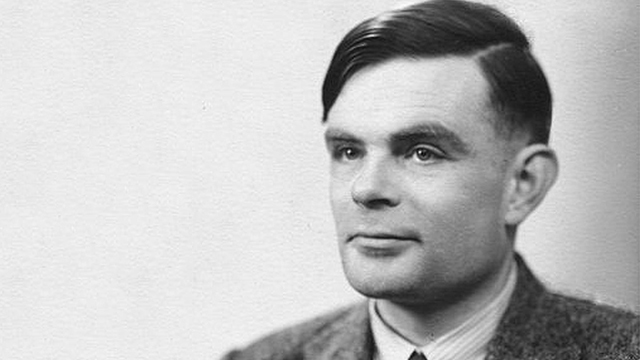
\includegraphics[height=3.3cm]{./images/Turing.jpg}
  \end{center}
 ~\\
 
\dgold{\emph{On Computable Numbers, with an Application to the Entscheidungsproblem} (1936)}\\
 
 \cinza{(computability and the birth of computer science)}

\end{block}

\end{slide}

%----------------------------------------------------------------------------------
\begin{slide}{The subject}
\small

\begin{block}{Richard Feynman (1918 - 1988)}
\begin{center}
 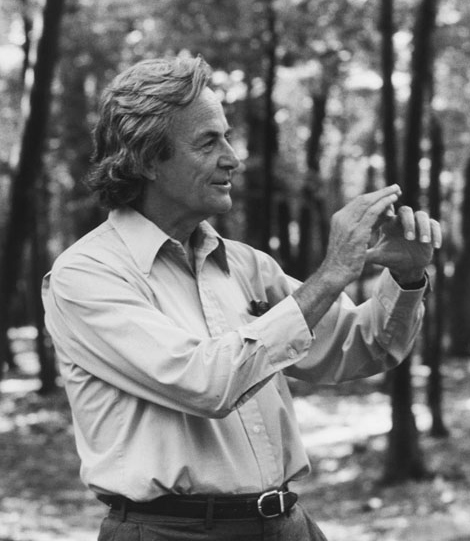
\includegraphics[height=3.3cm]{./images/Feynman1984.jpg}
  \end{center}
 ~\\
 
\dgold{\emph{Simulating Physics with Computers} (1982)}\\
 
 \cinza{(quantum reality as a computational resource)}

\end{block}

\end{slide}


%----------------------------------------------------------------------------------
\begin{slide}{The subject}
\small

\begin{block}{Davis Deutsch (1953)}
\begin{center}
 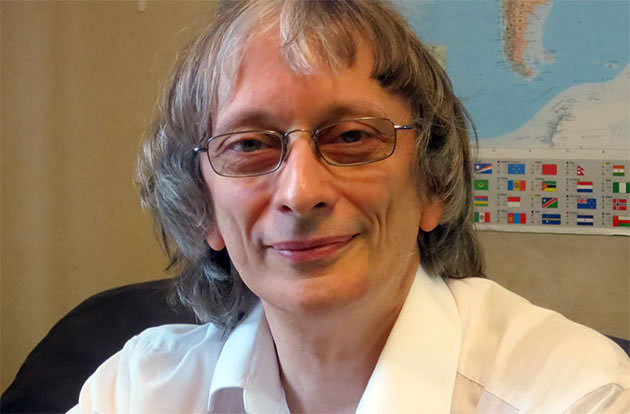
\includegraphics[height=3.3cm]{./images/DeutschD.jpeg}
  \end{center}
 ~\\
 
\dgold{\emph{Quantum theory, the Church-Turing principle and the universal quantum computer} (1985)}\\
 
 \cinza{(quantum computability and computational model: \\ first example of a quantum algorithm that is exponentially faster than any possible deterministic classical one)}

\end{block}

\end{slide}

%----------------------------------------------------------------------------------
\begin{slide}{The subject}
\small
\vspace{0.1cm}
%
\begin{center}
\begin{equation*}
\xymatrix{
\text{\emph{\dkb{quantum resources}}} & \text{\emph{\dkb{quantum algorithms}}} & \text{\emph{\dkb{computability}}}&\\
  \text{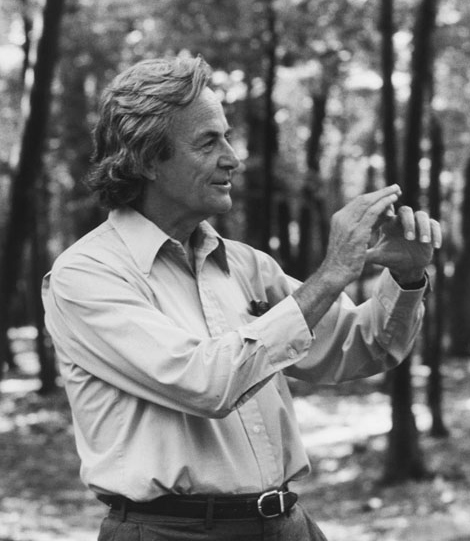
\includegraphics[height=2cm]{./images/Feynman1984.jpg}}%\hspace{0.1cm}}
 \ar[rd] &
 \text{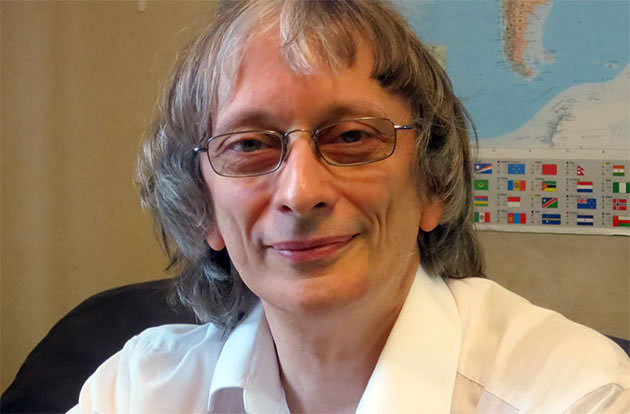
\includegraphics[height=2cm]{./images/DeutschD.jpeg}}%\hspace{0.1cm}}
  \ar[d] &
\text{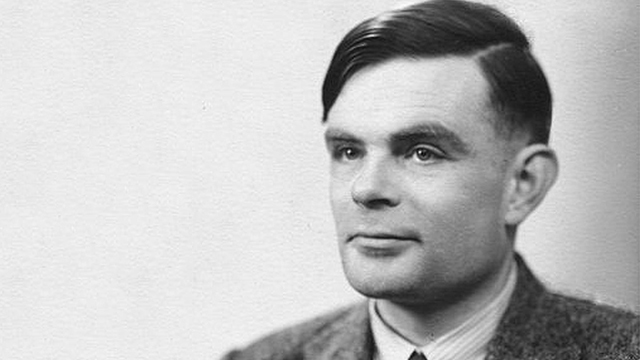
\includegraphics[height=2cm]{./images/Turing.jpg}}
 \ar[ld] \\
& &
 &
 }
\end{equation*}
\end{center}

 
 \end{slide}
%----------------------------------------------------------------------------------
\begin{slide}{The subject}
\small
\vspace{0.1cm}
%
\begin{center}
\begin{equation*}
\xymatrix{
\text{\emph{\dkb{quantum resources}}} & \text{\emph{\dkb{quantum algorithms}}} & \text{\emph{\dkb{computability}}}&\\
  \text{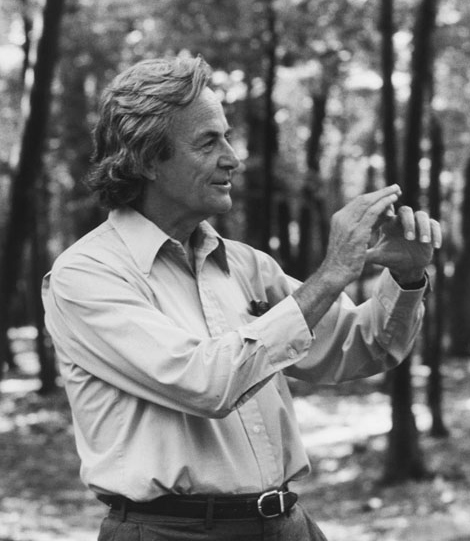
\includegraphics[height=2cm]{./images/Feynman1984.jpg}}%\hspace{0.1cm}}
 \ar[rd] &
 \text{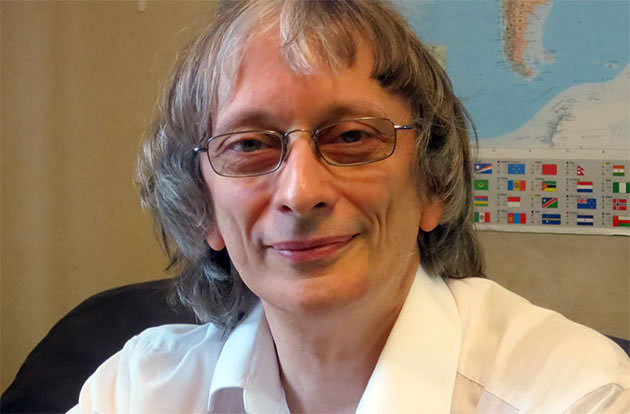
\includegraphics[height=2cm]{./images/DeutschD.jpeg}}%\hspace{0.1cm}}
  \ar[d] &
\text{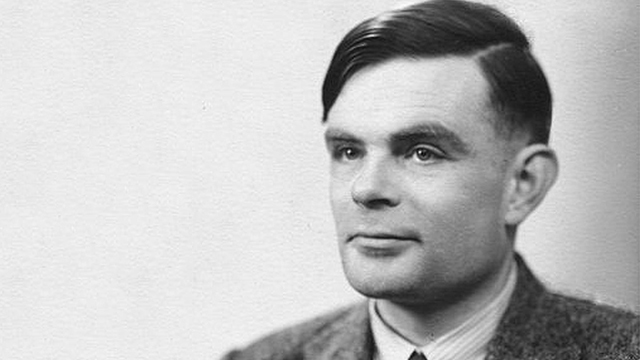
\includegraphics[height=2cm]{./images/Turing.jpg}}
 \ar[ld] \\
& &
%\text{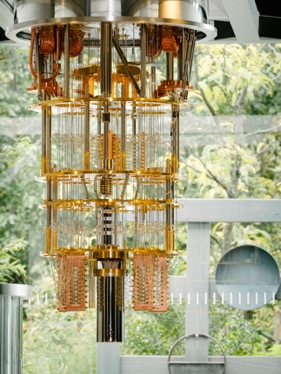
\includegraphics[height=2cm]{./images/ibmq.jpg}} &
 }
\end{equation*}
\end{center}

\vspace{-0.5cm}
\begin{center}
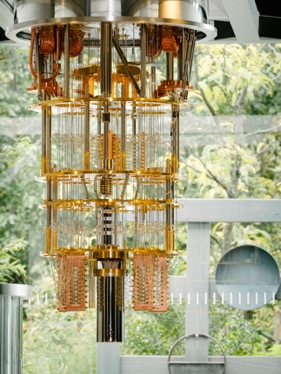
\includegraphics[height=2.3cm]{./images/ibmq.jpg}
\end{center}

 
 \end{slide}


 
 %----------------------------------------------------------------------------------
\begin{slide}{The subject}
\small
\vspace{0.1cm}
%
\begin{center}
\begin{equation*}
\xymatrix{
\text{\emph{\dkb{quantum resources}}} & \text{\emph{\dkb{quantum algorithms}}} & \text{\emph{\dkb{computability}}}&\\
  \text{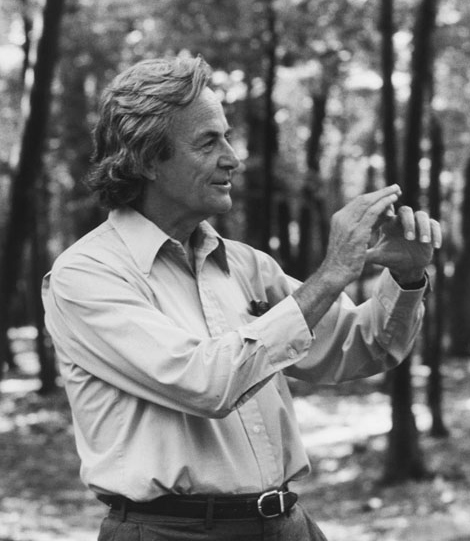
\includegraphics[height=2cm]{./images/Feynman1984.jpg}}%\hspace{0.1cm}}
 \ar[rd] &
 \text{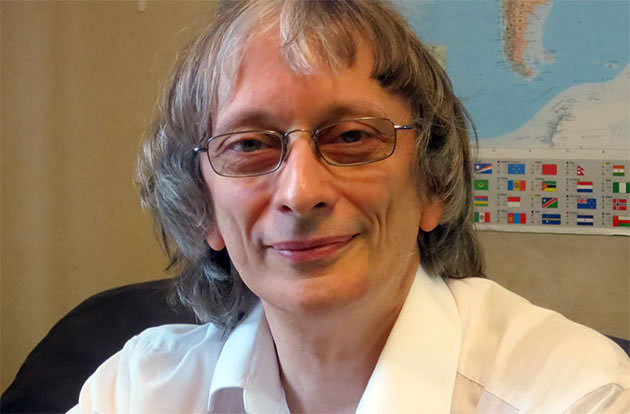
\includegraphics[height=2cm]{./images/DeutschD.jpeg}}%\hspace{0.1cm}}
  \ar[d] &
\text{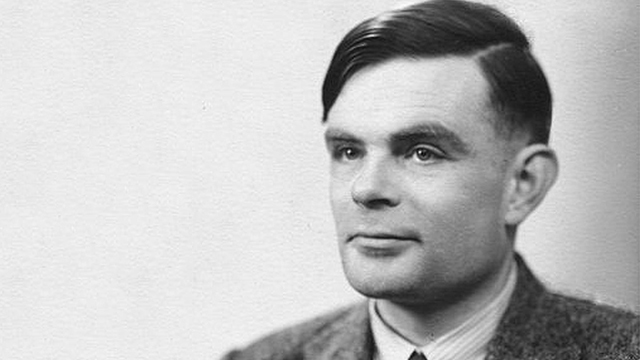
\includegraphics[height=2cm]{./images/Turing.jpg}}
 \ar[ld] \\
& &
%\text{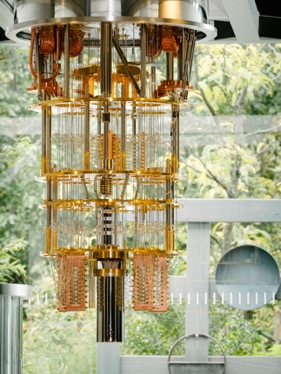
\includegraphics[height=2cm]{./images/ibmq.jpg}} &
 }
\end{equation*}
\end{center}

 

\vspace{-0.5cm}
\begin{center}
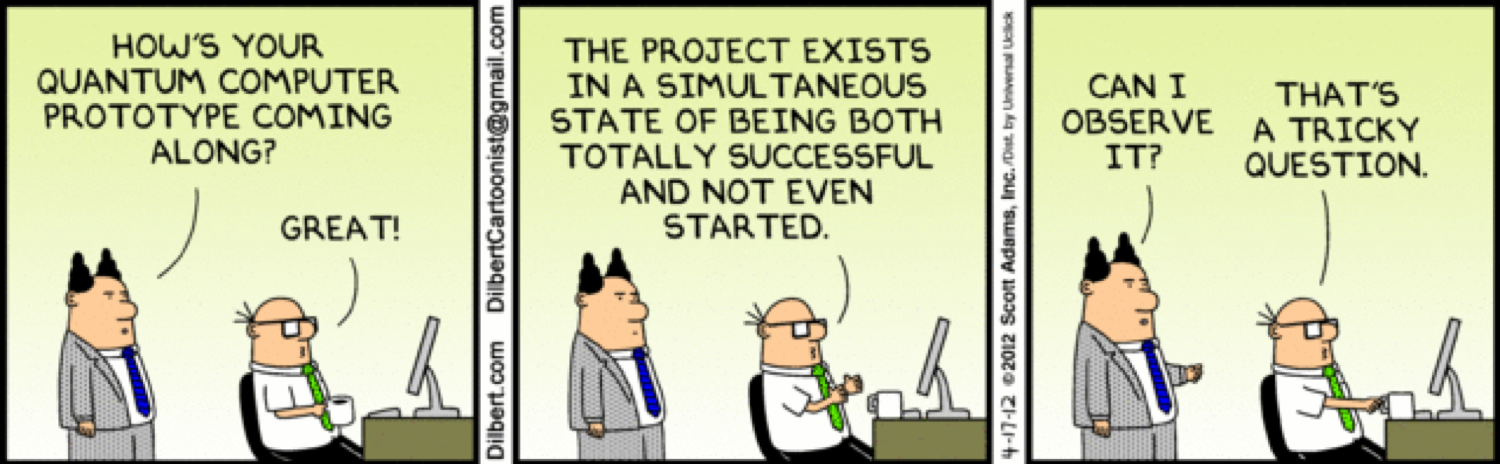
\includegraphics[height=2.3cm]{./images/Quantuncaortoon.png}
\end{center}
 \end{slide}


 %----------------------------------------------------------------------------------
\begin{slide}{Quantum is trendy ...}
\small
 
 \begin{block}{The second quantum revolution}
For the first time the viability of quantum computing may be \dkb{demonstrated in a number of real problems} extremely difficult to handle, if possible at all, classically, and \dkb{its utility discussed across industries}. 

\begin{itemize}
\item \dkb{huge investment} by both the States, large companies and startups
\item the \dkb{race for quantum} rising between major IT players \\ (e.g. IBM, Intel, Google, Microsoft)
\item \dkb{proof-of-concept machines} up to 50 qubits until the end of 2018 
\item \dkb{national and regional programmes} \\ (from the 2016 Quantum Manifesto to the  EU QT Flagship)
\end{itemize}



\end{block}
\end{slide}

%----------------------------------------------------------------------------------
\begin{slide}{... but the race is just starting}
\small



\begin{center}
\begin{tabular}{cc}
 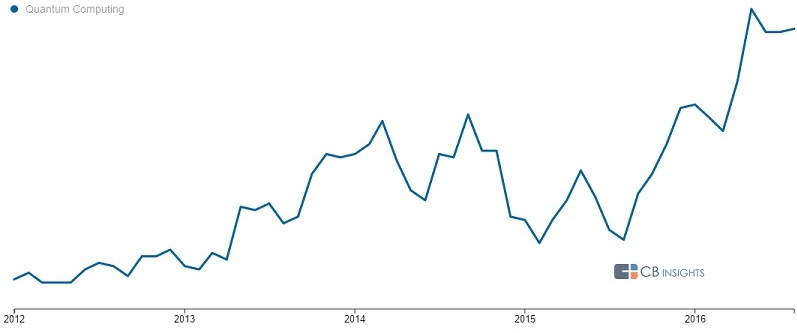
\includegraphics[height=2.2cm]{./images/QC-ref} &  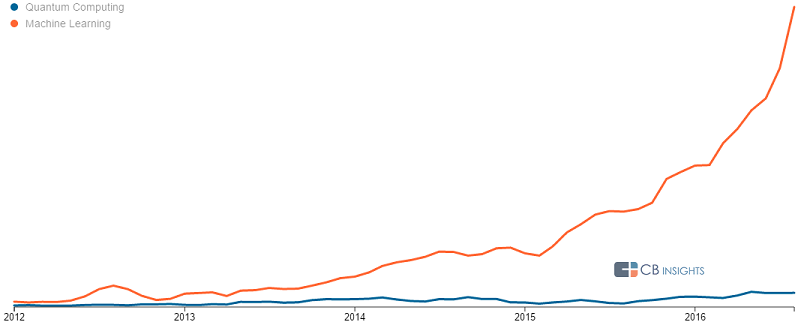
\includegraphics[height=2.2cm]{./images/QC-ML-ref}
 \end{tabular}
 \end{center}
 
 \begin{itemize}
 \item Clearly, quantum computing will have a \dkb{substantial impact on societies} even if, being a so \dkb{radically different
technology},
\item ...   it is difficult to \dkb{anticipate 
its  evolution} and future applications ...
\item ... and  its \dkb{commercial potential} in� the  near term (5 to 10 yrs) is still debatable
\end{itemize}

\end{slide}

%----------------------------------------------------------------------------------
\begin{slide}{Where exactly do we stand?}
\small

 \begin{block}{Short term}
Quantum advantage with \dkb{Noisy Intermediate-Scale Quantum} (NISQ) \\
\dkb{Hybrid} computational models: 
\begin{itemize}
\item the quantum device as a coprocessor
\item typically accessed as a service over the cloud %, maybe for a fee, ideally enforced for commercial reasons 
\end{itemize}
 \end{block}
 
 \begin{center}
 \begin{tabular}{cc}
  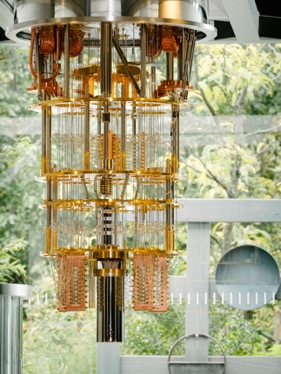
\includegraphics[height=4cm]{./images/Picture1.jpg} & 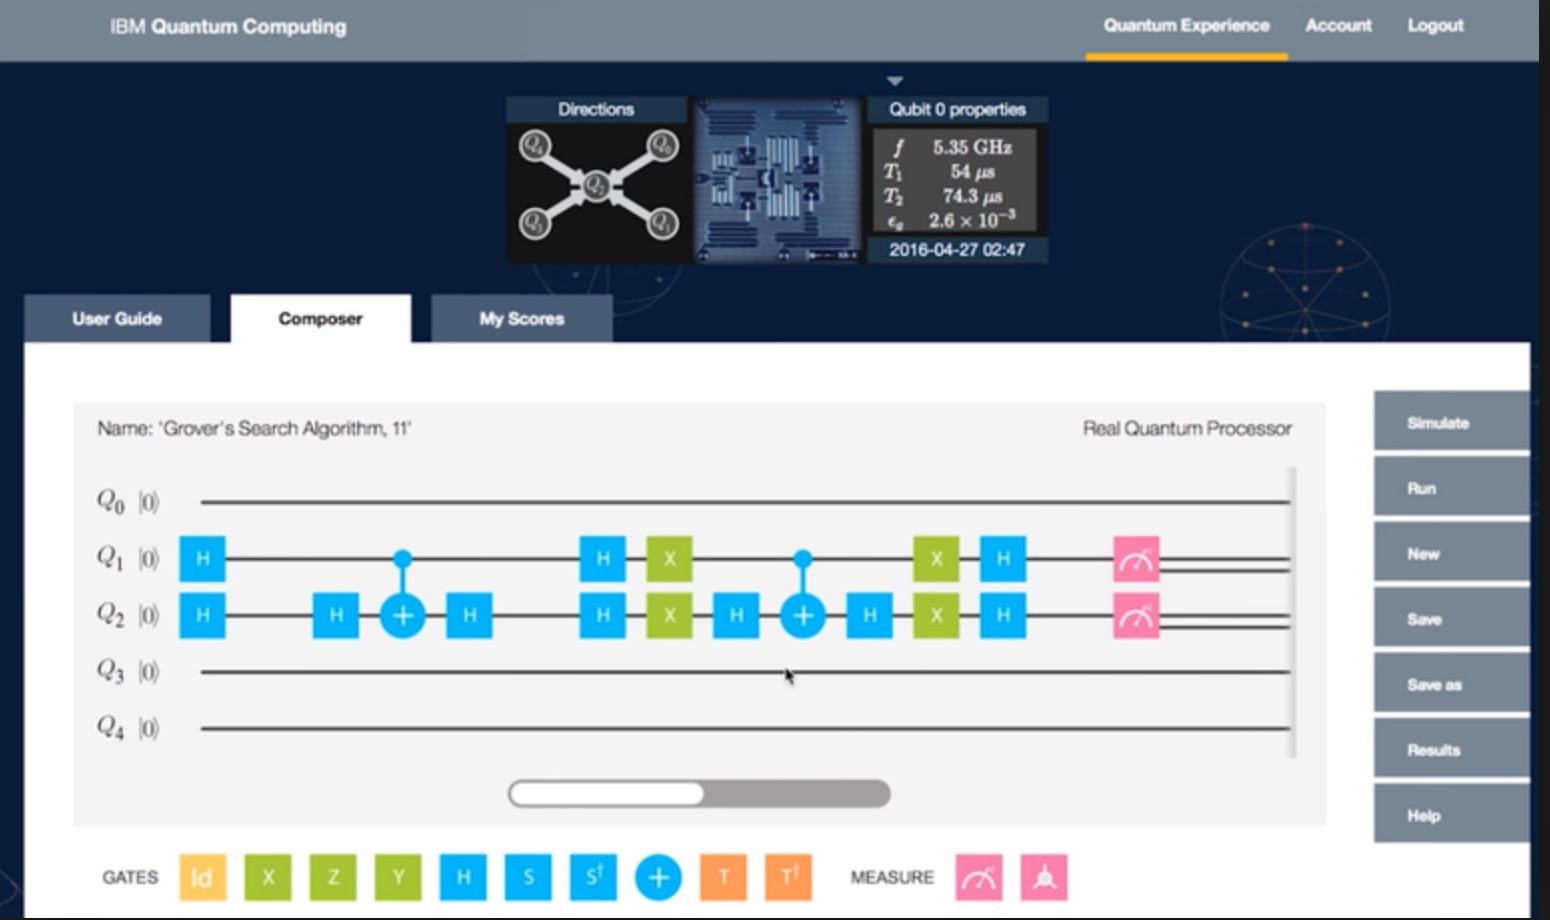
\includegraphics[height=4cm]{./images/ibmcirc}
 \end{tabular}
 \end{center}
 \end{slide}



%----------------------------------------------------------------------------------
\begin{slide}{Where exactly do we stand?}
\small

 \begin{block}{Longer term}
 \dkb{Fault tolerant} quantum computing, base on error correction codes (using millions of physical qubits to implement a logic one)
\end{block}


\begin{block}{From now to then there is a need for }
\begin{itemize}
\item basic research (in several fronts), but also
\item use cases
\item capacity building
\item process re-engineering 
\item anticipating social impacts and challenges
\end{itemize}
\end{block}

 \end{slide}
 
%----------------------------------------------------------------------------------
\begin{slide}{Learning Outcomes}
\small

On successful completion  of the course students should be able

\begin{itemize}
\item To understand basic concepts of computability, computational complexity, and underlying mathematical structures;
\item To master the quantum computational model;
\item To  design and analyse quantum algorithms;
\item To implement and run quantum algorithms in functional programming languages (Quipper) and the \qiskit\ development kit for IBM  Q quantum processors.
\end{itemize}

\end{slide}




%----------------------------------------------------------------------------------
\begin{slide}{Course Information and Pragmatics}
\small

\begin{block}{Refer to the course website at}
\begin{center}
\texttt{arca.di.uminho.pt/quantum-computation-2122/}
\end{center}
\end{block}


\end{slide}


%%----------------------------------------------------------------------------------
%\begin{slide}{Invitation to a fast running train ...}
%\small
%
%\vspace{0.2cm}
%\begin{block}{Academic IBM Q HUB since September, 1, 2018}
%\begin{itemize}
%\item Part of the worldwide IBM Q Network of companies and academies
%to exploit potential applications of Quantum Computing in Industry
%\item Real time, full access to new quantum machines
%\item Multidisciplinar, dedicated  teams
%\item A problem-driven research
%\item International cooperation 
%\end{itemize}
%\vspace{-1cm}
%\begin{flushright}
%
\includegraphics[height=3cm]{./images/qlab.jpg}
%\end{flushright}
%
%\end{block}
%\end{slide}
\end{document}



\end{document}


